\documentclass{scrartcl}
\usepackage[top=3cm, bottom=3cm, left=2cm,right=2cm]{geometry} 

\usepackage[english]{babel}
\usepackage[utf8]{inputenc}
\usepackage{mathtools}
\usepackage{esvect}
\usepackage{amssymb}
\usepackage{amsmath}

\usepackage{dcolumn}
\usepackage{booktabs}
\usepackage{tikz}
\usepackage{graphicx}
\usepackage{multicol}
\usepackage{float}
\usepackage{url}

\usepackage{listings}

%multiline comments
\usepackage{verbatim}

\usetikzlibrary{positioning,shapes,arrows}

\DeclareMathOperator*{\argmin}{argmin} % no space, limits underneath in displays
\DeclareMathOperator*{\argmax}{argmax} % no space, limits underneath in displays

\DeclarePairedDelimiter\abs{\lvert}{\rvert}%
\DeclarePairedDelimiter\norm{\lVert}{\rVert}%

\usepackage{titlesec}
\newcommand{\sectionbreak}{\clearpage}

\usepackage[parfill]{parskip}
\parskip = 4pt

\title{Künstliche Intelligenz 2 - Summary}
\author{Sebastian Rietsch}

\begin{document}
\maketitle

\section{Probablistic Reasoning, Part I: Basics}
\subsection{Introduction}
\textbf{Sources of Uncertainty} in Decision-Making:
\begin{itemize}
    \item
        Non-deterministic actions
    \item
        Partial observability with unreliable sensors
    \item
        Uncertainty about the domain behavior
\end{itemize}

What is \textbf{probabilistic reasoning}?
\begin{itemize}
    \item
        Deducing probabilities from knowledge about \textit{other} probabilities
    \item
        Determines probabilities that are difficult to assess, based on probabilities that are (relatively) easy to assess (\textit{to asses:} the process of estimating a probability \(P\) using statistics)
\end{itemize}

\textbf{Rational Agents}:
\begin{itemize}
    \item
        We have a choice of \textbf{actions}
    \item
        These can lead to different solutions with different probabilities
    \item
        The actions have different costs
    \item
        The results have different utilities
    \item
        A rational agent chooses the action with the \textbf{maximum expected utility}
\end{itemize}

\subsection{Unconditional Probabilities}
A \textbf{probability theory} is an assertion language for talking about possible worlds and an inference method for quantifying the degree of belief in such assertions (Example: we roll two dice with six sides, then we have 36 possible worlds: \((1,1), (2,1), \dots, (6,6)\)).

A \textbf{probability model} \(\langle \Omega, P \rangle\) consists of a set \(\Omega\) of possible worlds called the sample space and a probability function \(P: \Omega \rightarrow \mathbb{R}\), such that \(0 \leq P(\omega) \leq 1\) for all \(\omega \in \Omega\) and \(\sum_{\omega \in \Omega} P(\omega) = 1\). We restrict ourselves to a discrete, countable sample space.

\textbf{Random variables}:
\begin{itemize}
    \item
        A random variable is a variable quantity whose value depends on possible outcomes of unknown variables and processes we do not understand
    \item
        Given a random variable \(X\), \(P(X = x)\) denotes the prior probability, or unconditional probability, that \(X\) has value \(x\)
    \item
        We will refer to the fact \(X = x\) as an event or outcome
    \item
        For Boolean variable \(Name\), we write name for \(Name = \top\) and \(\lnot name\) for \(Name = \bot\)
\end{itemize}

The \textbf{probability distribution} for a random variable \(X\), written \(P(X)\), is the vector of probabilities for the (ordered) domain of \(X\).

Given a subset \(Z \subseteq \{X_1, \dots, X_n\}\) of random variables, an event is an assignment of values to the variables in \(Z\). The \textbf{joint probability distribution}, written \(P(Z)\), lists the probabilities of all events.

An \textbf{atomic event} is an assignment of values to all variables.

A \textbf{proposition} describes a set of multiple atomic events (\textbf{Example:} we roll two dice and are interested in the cases where they add up to 11). The probability associated with a proposition is defined by the sum of probabilities of the worlds in which it holds: For any proposition \(\phi, P(\phi) = \sum_{\omega \in \phi} P(\phi)\).

\textbf{Kolmogorov axioms:}
\begin{enumerate}
    \item
        The probability of an event is a non-negative real number: \[P(E) \in \mathbb{R}, P(E) \geq 0, \forall E \in F\] where \(F\) is the event space.
    \item
        The probability that at least one of the elementary events in the entire sample space will occure is 1: \(P(\Omega) = 1\).
    \item
        Any countable sequence of disjoint sets (mutually exclusive events) \(E_1, E_2, \dots \) satisfies \[P(\bigcup_{i=1}^{\infty} (E_i)) = \sum_{i=1}^{\infty} P(E_i).\]
\end{enumerate}
From this follows \(P(A \lor B) = P(A) + P(B) - P(A \land B)\).

\subsection{Conditional Probabilities}
In the presence of additional information, we can no loger use the unconditional (\textbf{prior}) probabilities (because probabilies model our belief, thus they depend on our knowledge).

Given propositions \(A\) and \(B\), \(P(a|b)\) denotes the \textbf{conditional probability} of \(a\) given that all we know is \(b\). The conditional, or posterior probability of \(a\) given \(b\) is defined as:
\[P(a|b) = \frac{P(a \land b)}{P(b)}\]

The \textbf{conditional probability distribution} of \(P(X|Y)\) is the table of all conditional probabilies of values of \(X\) given values of \(Y\).

\subsection{Independence}
Problem with full joint probility distributions: Given \(n\) random variables with \(k\) values each, the joint pdf containts \(k^n\) probabilities. This motivates the use of conditional probabilities while exploiting the \textbf{(conditional) independence} property.

Events \(a\) and \(b\) are \textbf{independent} if \(P(a \land b) = P(a) \cdot P(b)\), from which follows that \(P(a | b) = P(a)\) and vice versa.

In case of independence, the joint probability distribution of multiple variables can be reconstructed from smaller, statistically independent joint probability distributions.

\subsection{Basic Probabilistic Reasoning Methods}
\begin{itemize}
    \item
        \textbf{Product Rule:} \(P(a \land b) = P(a | b) P(b)\) 
    \item
        \textbf{Chain Rule:} \(P(X_1, \dots, X_n) = P(X_n | X_{n-1}, \dots X_1) \cdot \dots \cdot P(X_2 | X_1) \cdot P(X_1)\) (This works for any ordering of the variables)
    \item
        \textbf{Marginalization:} Given sets \(X\) and \(Y\) of random variables, we have:
        \[P(X) = \sum_{y \in Y} P(X, y)\]
    \item
        \textbf{Normalization:} Given a vector \(\langle w_1, \dots, w_k \rangle\) of numbers in \([0,1]\) where \(\sum_{i=1}^k w_i \leq 1\), the normalization constant \(\alpha\) is \(\alpha \langle w_1, \dots, w_k \rangle = 1/\sum_{i=1}^k w_i\)
        \begin{itemize}
            \item
                Given a random variable \(X\) and an event \(e\), we have \(P(X|e) = \alpha P(X, e)\) with \(\alpha = 1/P(e)\)
            \item
                Normalization + Marginalization: Given "query variable" \(X\), "observed event" \(e\), and "hidden variables" set \(Y\):
                \[P(X|e) = \alpha P(X, e) = \alpha \sum_{y \in Y} P(X, e, y)\]
        \end{itemize}
\end{itemize}

\subsection{Bayes' Rule}
Given propositions \(A\) and \(B\) where \(P(a) \neq 0\) and  \(P(b) \neq 0\), we have:
\[P(a|b) = \frac{P(b|a) P(a)}{P(b)}\]

\subsection{Conditional Independence}
Given sets of random variables \(Z_1, Z_2 \text{ and } Z\), we say \(Z_1\) and \(Z_2\) are \textbf{conditionally independent given \(Z\)} if:
\[P(Z_1, Z_2 | Z) = P(Z_1 | Z) \cdot P(Z_2 | Z)\]

If \(Z_1\) and \(Z_2\) are conditionally independent given \(Z\), the \(P(Z_1 | Z_2, Z) = P(Z_1 | Z)\).

\subsection{Summary}
\begin{itemize}
    \item
        Uncertainty is unavoidable in many environsments, namely whenever agents do not have perfect knowledge
    \item
        Probabilities express the degree of belief of an agent, given its knowledge, into an event
    \item
        Conditional probabilities express the likelihood of an event given observed evidence
    \item
        Assessing a probability means to use statistics to approximate the likelihood of an event
    \item
        Bayes' rule allows us to derive, from probabilities that are easy to assess, probabilities that arn't easy to assess
    \item
        Given mulitple evidence, we can exploit conditional independencie
\end{itemize}

\section{Probabilistic Reasoning, Part II: Bayesian Networks}
\subsection{What is a Bayesian Network}
Given random variables \(X_1, \dots, X_n\) with finite domains \(D_1, \dots, D_n\), a \textbf{Bayesian network} is an acyclic directed graph \(BN = \langle \{X_1, \dots, X_n\}, E\rangle\). We denote \(Parents(X_i) = \{X_j | (X_j, X_i) \in E \}\). Each \(X_i\) is associated with a function \(CPT(X_i): D_i \times \prod_{X_j \in Parents(X_i)} D_j \rightarrow [0,1]\), the \textbf{conditional probability table}. Is is a so called \textbf{graphical model}.

A node \(X\) is conditionally independent of its non-descendants (nicht Nachkommen) given its parents. A node \(X\) is conditionally independent of all other nodes in the network given its Markov blanket (parents, children, and children's parents).

\subsection{Recovering the Full Joint Probability Distribution}

\textbf{Chain rule:} For any ordering \(X_1, \dots, X_n\) we have
\[P(X_1, \dots, X_n) = P(X_n | X_{n-1} \dots, X_1) \cdot P(X_{n-1} | X_{n-2} \dots, X_1) \dots P(X_1)\]
Choose \(X_1, \dots, X_n\) consistent with \(BN: X_j \in Parents(X_i) \Rightarrow j<i\) 

With \(BN\) assumption, we can use \(P(X_i|Parents(X_i))\), instead of \(P(X_i| X_{i-1} \dots X_1)\):
\[P(X_1, \dots, X_n) = \prod_{i=1}^n P(X_i | Parents(X_i))\]

\subsection{Constructing Bayesian Networks}
Reminder: Conditional Independence 

Events \(R\) and \(B\) are conditionally independent given \(Y\) if and only if \(P(R, B | Y) = P(R|Y)P(B|Y)\) or equivalently \(P(R|B,Y) = P(R|Y)\).

\bigbreak

A Bayesian network is only a correct representation of a domain if each node is conditionally independent of its other predecessors (Vorfahren) in the node ordering, given its parents. We can satisfy this condition with this methodology:
\begin{enumerate}
    \item
        Nodes: First determine the set of variables that are required to model the domain. Now order them, \(X_1, \dots, X_n\). Any order will work, but the resulting network will be more compact if the variables are orderes such that cuases precede effects. 
    \item
        Links: For \(i=1\) to \(n\) do:
        \begin{itemize}
            \item
                Choose, from \(X_1, \dots, X_{i-1}\) a minimal set of parents for \(X_i\), such that conditional dependence is satisfied
            \item
                For each parent insert a link from parent to \(X_i\) 
            \item
                CPTs: Write down \(P(X_i|Parents(X_i))\) 
        \end{itemize}
\end{enumerate}

\bigbreak

The size on a Bayesian Network \(size(BN)\) is defined as the total number of entries in the CPTs. Bayesian Networks are compact is each variable is directly influenced by only a few of its predecessor variables.

\subsection{Efficient Representation of Conditional Distributions}
Even if the maximum number of parents \(k\) is smallish, filling in the CPT for a node requires up to \(O(2^k)\) numbers and perhaps a great deal of experience with all the possible conditioning cases.

\textbf{Deterministic node:} has its value specified exactly by the values of its parents, with no uncertainty \(\Rightarrow\) no explicit CPT needed

\bigbreak

Uncertain relationships can often be characterized by so-called noisy logical relationships, where the \textbf{noisy-OR} relation is the standard example (a good exmaple is the relationship between diseases and symptoms).

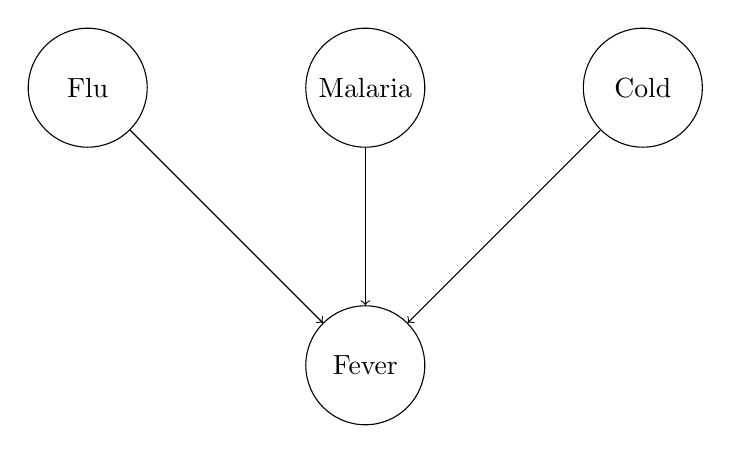
\begin{tikzpicture}[
  node distance=2cm and 2cm,
  mynode/.style={draw,circle,text width=1.2cm,align=center},
]
\node[mynode] (flu) {Flu};
\node[mynode,right=of flu] (malaria) {Malaria};
\node[mynode,right=of malaria] (cold) {Cold};
\node[mynode,below=of malaria] (fever) {Fever};

\path (flu) edge[->] (fever)
(malaria) edge[->] (fever)
(cold) edge[->] (fever)
;
\end{tikzpicture}

The causal relationship between parent and child may be inhibited (e.g. no fever but has flu). Two assumptions:
\begin{itemize}
    \item
        All the possible causes are listed (If some are missing, we can always add a so-called leak node that covers "miscellaneous causes")
    \item
        Inhibition of each parent is independent of any other parent (Whatever inhibits malaria from causing a fever is independet of whatever inhibits flu from causing fever)
\end{itemize}
Given these assumptions, \(Fever\) is false if and only if all its \(true\) parents are inhibited

\(\Rightarrow P(x_i | parents(X_i)) = 1 - \prod_{j:X_j = true} q_j\), where \(q_j\) are the inhibition probabilities.

The full CPT can now be described using \(O(k)\) parameters.

\subsection{Inference in Bayesian Networks (Inference by enumeration)}
The basic task for any probabilistic inference system is to compute the posterior probability distritubtion for a set of \textbf{query variable}(s) \(X\), given some observed \textbf{event} \(e\) - that is, some assignment of values to a set of \textbf{evidence variables} \(E = \{E_1, \dots, E_m\}\). \(Y = \{Y_1, \dots, Y_l\}\) will denote the nonevidence, nonquery variables, also called \textbf{hidden variables}.

\bigbreak

Conditional probabilities can be computed by summing terms from the full joint probability distribution:
\[P(X|e) = \alpha P(X, e) = \alpha \sum_y P(X, e, y)\]
\textit{Reminder:} \(P(X|e) = \frac{P(X,e)}{P(e)} = \alpha P(X,e),\ \alpha = \frac{1}{P(e)}\)

A query can be answered using a Bayesian network by computing sums of products of conditional probabilities from the network.

\textit{Reminder:} \(P(X_1, \dots, X_n) = \prod_{i=1}^n P(X_i | Parents(X_i))\)

\bigbreak

\textbf{Example} (hidden variables: \textit{Earthquake} and \textit{Alarm}):
\begin{align*}
    P(Burglary | JohnCalls = \top, MaryCalls = \top) = P(B | j, m) &= \alpha \sum_e \sum_a P(B, j, m, e, a) \\
    &= \alpha \sum_e \sum_a P(b) P(e) P(a|b,e) P(j|a) P(m|a)\\
    &= \alpha P(b) \sum_e P(e) \sum_a  P(a|b,e) P(j|a) P(m|a)
\end{align*}


\textbf{Variable Elimnation} can make computation increadibly faster in the case of polytrees (there is at most one undirected path between any two nodes in the graph).

General probabilistic inference is \(\#P\)-hard, which is harder then NP. In the hard cases, approxiamation is key.

\subsection{Conclusion}
\begin{itemize}
    \item
        \textbf{Bayesian networks} are a wide-spread tool to model uncertainty, and to reason about it. A BN represents \textbf{conditional independence} relations between random variables. It consists of a graph encoding the variable dependencies, and of conditional probability tables (CPTs).
    \item
        Given a variable order, the BN is small (concerning CPT sizes) if every variable depends only on a few of its predecessors
    \item
        \textbf{Probabilistic inference} requires to compute the probability distribution of a set of query variables, given a set of evidence variables whose values we know. The remaining variables are hidden. 
    \item
        Inference by enumeration takes a BN as input, then applies \textbf{Normalization and Marginalization}, the \textbf{Chain rule}, and exploits conditional independence.
    \item
        \textbf{Variable elimination} avoids unnecessary computation. It runs in polynomial time for polytree BNs. In general, exact probabilistic inference is \(\#P-hard\). Approximate probabilistic inference methods exist.
\end{itemize}

\section{Making Simple Decisions Rationally}
\subsection{Rational Preference}
\textbf{Decision theory} investigates how an agent \(a\) deals with choosing among actions based on the desirability of their outcomes. We restrict ourself to \textbf{episodic} decision theory, which deals with choosing among actions based on the desirabilty of their immediate outcomes. We have to deal with non-deterministic, partially observable environments.

\bigbreak

\(Result(a)\) is a random variable, whose values are possible outcome states of an action. The probability of outcome \(s'\), given evidence observations \(e\), is written
\(P(Result(a) = s' | a,e)\).

The agent's preferences are captured by a \textbf{utility function} \(U(s)\), which assigns a single number to express the desirability of a state. The \textbf{expected utility} of an action given the evidence, \(EU(a|e)\), is just the average utility value of the outcomes, weighted by the probability that the outcome occurs:
\[EU(a|e) = \sum_{s'} P(Result(a) = s'|a,e)U(s')\]

The principle of \textbf{maximum expected utility} (MEU) says that a rational agent should choose the action that maximizes the agent's expected utility:
\[action = argmax_a EU(a|e)\]

\subsubsection{Preference}
An agent chooses among \textbf{outcomes} (\(A, B\), etc.) and \textbf{lotteries}, i.e., situations with uncertain prizes.
\[Lottery \ L = [p_1, S_1; p_2, S_2; \dots p_n, S_n]\]
\begin{itemize}
    \item
        \(A \succ B\): \(A\) \textbf{preffered} over \(B\)
    \item
        \(A \sim B\): \textbf{indifference} between \(A\) and \(B\)
    \item
        \(A \succeq B\): \(A\) prefered over \(B\) or indifferent
\end{itemize}
Six constraint that we require any reasonable preference relation to obey: Orderability, Transitivity, Continuity, Substituability, Monotonicity, Decomposability (Axioms of utility theory).
%\begin{itemize}
 %   \item
 %       Orderability: Given any two lotteries, a rational agent either prefer one to the other or else rate the two as equally preferable.
 %   \item
 %       Transitivity: If an agent prefers \(A\) over \(B\) and \(B\) over \(C\), then the agent must prefer \(A\) over \(C\).
 %   \item
%        Continuity: If some lottery \(B\) is between \(A\) and \(C\) in preference, then there is some probability \(p\) for which the rational agent will be indifferent between getting \(B\) for sure and the lottery that yields \(A\) which \(p\) and \(C\) with \(1-p\).
%    \item
%        Substituability: If an agent is indifferent between two lotteries \(A\) and \(B\), then the agent is indifferent between two more complex lotteries that are the same except that \(B\) is substituted for \(A\) in one of them: \(A \sim B \Rightarrow [p, A; 1-p, C] \sim [p, B; 1-p, C]\). This also holds if we substitute \(\succ\) for \(\sim\) in this axiom.
%    \item
%        Monotonicity: Suppose two lotteries have the same two possible outcomes
%\end{itemize}

\subsubsection{Preference lead to utility}
\begin{itemize}
    \item
        \textbf{Existence of Utility Function:} If an agent's preferences obey the axioms of utility, then there exists a function \(U\) such that \(U(A) > U(B)\) if and only if \(A\) is preferred to \(B\), and \(U(A) = U(B)\) if and only if the agent is indifferent between \(A\) and \(B\).\\
         \[U(A) > U(B) \Leftrightarrow A \succ B\]
    \item
        \textbf{Expected Utility of a Lottery:} The utility of a lottery is the sum of probability of each outcome times the utility of that outcome.
        \[U([p_1, S_1; \dots; p_n, S_n]) = \sum_i p_i U(S_i)\]
\end{itemize}
We call a total preference ordering on states a \textbf{value function} or \textbf{ordinal utility function}.

\textit{Note:} An agent doesn't implicitly have to maximize an utility function. Rational behavior can be generated in any number of ways. By observing a rational agent's preference, however, an observer can construct the utility function that represents what the agent is actually trying to achieve (even if the agent doesn't know it)

\subsubsection{Utility assessment and utility scales}
\underline{Goal:} working out a agent's utility function (\textbf{preference elicitation}). This process involves presenting choices to the agent and using the observed preferences to pin down the underlying utility function.

Fix the utility of a "best possible price" at \(U(S) = u_{\top}\) and a "worst possible catastrophe" at \(U(S) = u_{\bot}\). \textbf{Normalized utilities} use a scale with \(u_{\bot} = 0\) and \(u_{\top} = 1\).

Given a utility scale between \(u_{\bot}\) and \(u_{\top}\), we can assess the utility of any particular prize \(S\) by asking the agent to choose between \(S\) and a \textbf{standard lottery} \([p, u_{\top}; (1-p), u_{\bot}]\). The probability \(p\) is adjusted until the agent is indifferent between \(S\) and the standard lottery. Assuming normalized utilities, the utility of \(S\) is given by \(p\). Once this is done for each prize, the utilities for all lotteries involving those prizes are determined.

\subsection{Multiattribute Utility Functions}
Problems, in which outcomes are characterized by two or more attributes, are handled by \textbf{multiattribute utility theory}. We will call the attributed \(X = X_1, \dots, X_n\); a complete vector of assignments will be \(x = \langle x_1, \dots, x_n \rangle\), where each \(x_i\) is either a numeric or discrete value. We will assume that higher values of an attribute correspond to higher utilities.

\subsubsection{Dominance}
A choice \(S_1\) is said to \textbf{strictly} dominate \(S_2\), iff \(X_i(S_1) > X_i(S_2), \ \forall i\). For the non-deterministic case, all possible concrete outcomes for \(S_1\) have to strictly dominante all possible outcomes for \(S_2\) (very rare).

\begin{center}
    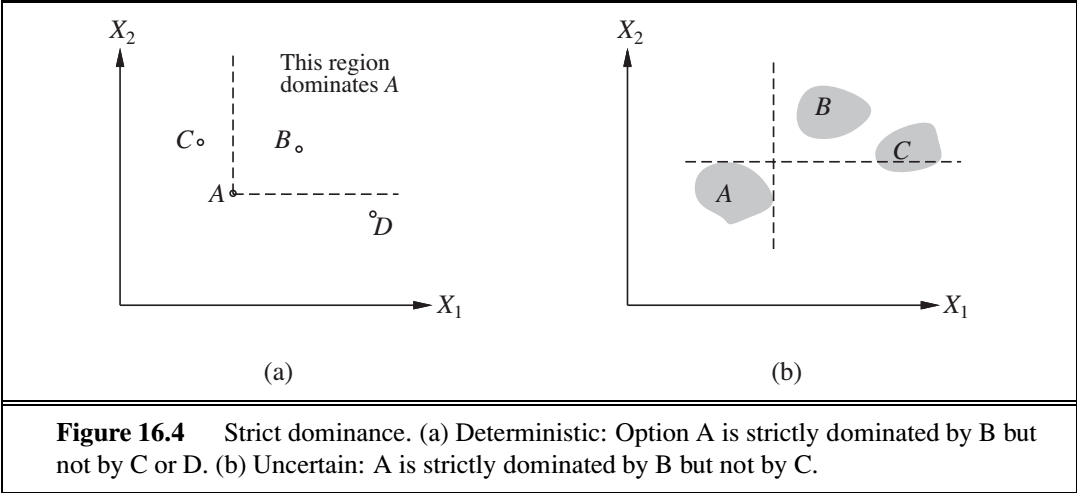
\includegraphics[scale=0.4]{img/stricdom.png}
\end{center}

If two actions \(A_1\) and \(A_2\) lead to probability distributions \(p_1(x)\) and \(p_2(x)\) on attribute \(X\), then \(A_1\) \textbf{statistically dominates} \(A_2\) if
\[\forall x \int_{-\infty}^x p_1(x') dx' \leq \int_{-\infty}^x p_2(x')dx'\]
(the cumulative distribution of \(S_1\) is always to the right of the one for \(S_2\)).

If \(A_1\) stochatically dominates \(A_2\), then for any monotonically nondecreaing utility function \(U(x)\), the expected utility of \(A_1\) is at least as high as the expected utility of \(A_2\). Hence, if an action is stochastically dominated by another action on all attributes, then it can be discarded.

\begin{center}
    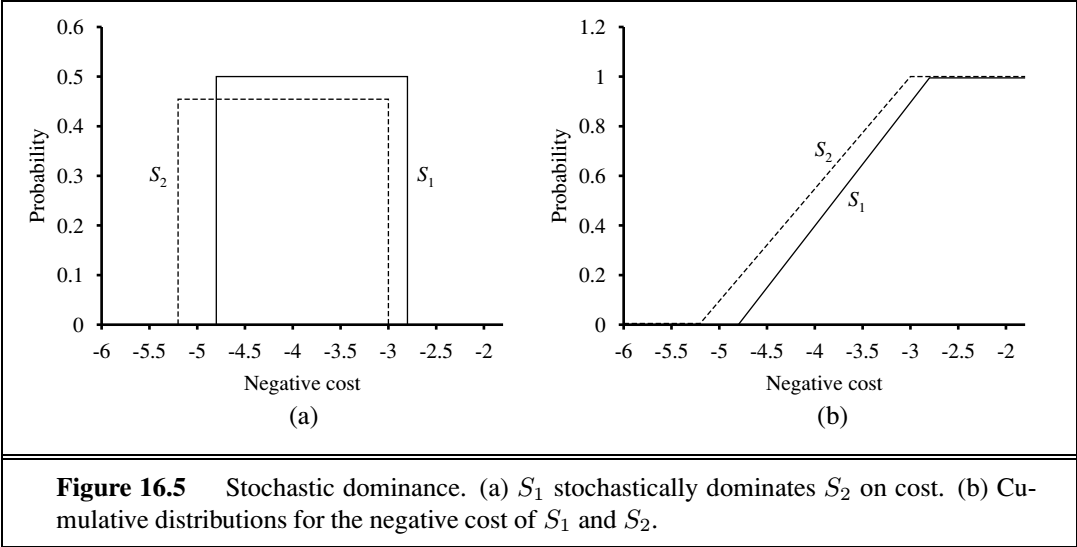
\includegraphics[scale=0.4]{img/statdom.png}
\end{center}

\subsubsection{Preference structure and multiattribute utility}
Suppose we have \(n\) attributes, each of which has \(d\) distinct possible values. To specify the complete utility function \(U(x_1, \dots, x_n)\), we need \(d^n\) values in the worst case. Now, the worst case corresponds to a situation in which the agent's preferences have no regularity at all. Multiattribute utility theory is based on the suppostition that the preferences of typical agents have much more structure than that.

The basic approach is to identify regularities in the preference behavior and to use what are called \textbf{representation theorems} to show that an agent with a certain kind of preference structure has a utility function
\[U(x_1, \dots, x_n) = F[f_1(x_1), \dots, f_n(x_n)]\]
where \(F\) is, we hope, a simple function such as addition.

... whatever (Was wollen sie mir hier genau beibringen Herr Kohlhase?)

\subsection{Decision Networks}
Decision networks combine Bayesian networks with additional node types for actions and utilities.

\subsubsection{Representing a decision problem with a decision network}
In it's most general form, a decision network represents information about the agent's current state, its possible actions, the state that will result from the agent's action, and the utility of that state.

\textbf{Node types:}
\begin{itemize}
    \item
        \textbf{Chance nodes} (oval) represent random variables. Each node has associated with it a conditional distribution that is indexed by the state of the parent nodes.
    \item
        \textbf{Decision nodes} (rectangle) represent points where the decision maker has a choice of actions.
    \item
        \textbf{Utility nodes:} (diamonds) represent the agent's utility function. The utility node has as parents all variables describing the outcome that directly affect utility. Associated with the utility node is a description of the agent's utility as a function of the parents attributes.
\end{itemize}

\begin{center}
    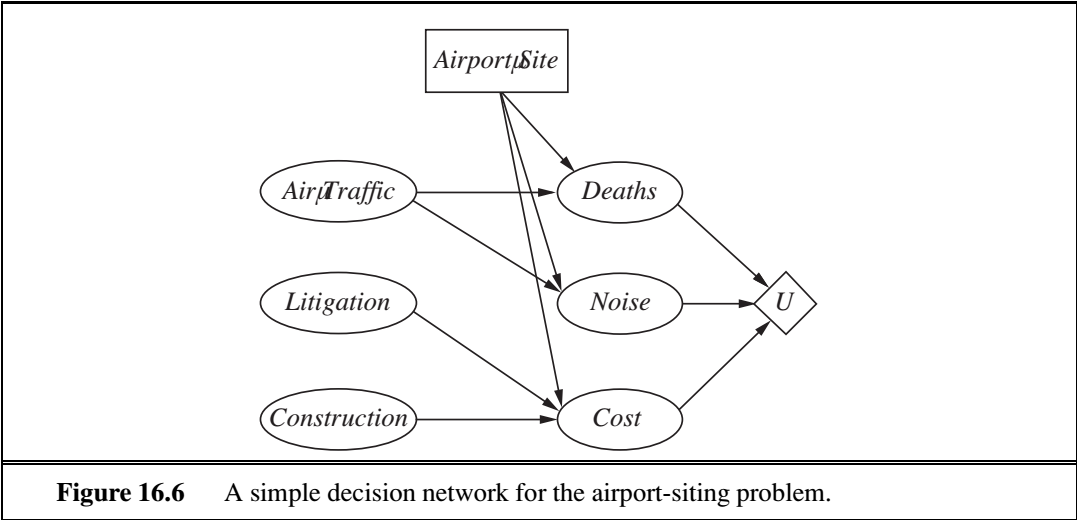
\includegraphics[scale=0.4]{img/airport.png}
\end{center}

Actions are selected by evaluating the decision network for each possible setting of the decision node. 
\textbf{Algorithm:}
\begin{enumerate}
    \item
        Set the evidence variables to the current state
    \item
        For each possible value of the decision node:
        \begin{enumerate}
            \item
                Set the decision node to that value
            \item
                Calculate the posterior probabilities for the parent nodes of the utility node, using a standard probabilistic inference algorithm
            \item
                Calculate the resulting utility for the action
        \end{enumerate}
    \item
        Return the action with the highest utility
\end{enumerate}

\begin{comment}
\subsection{Recap: Agent Architectures based on Belief States}
\begin{center}
    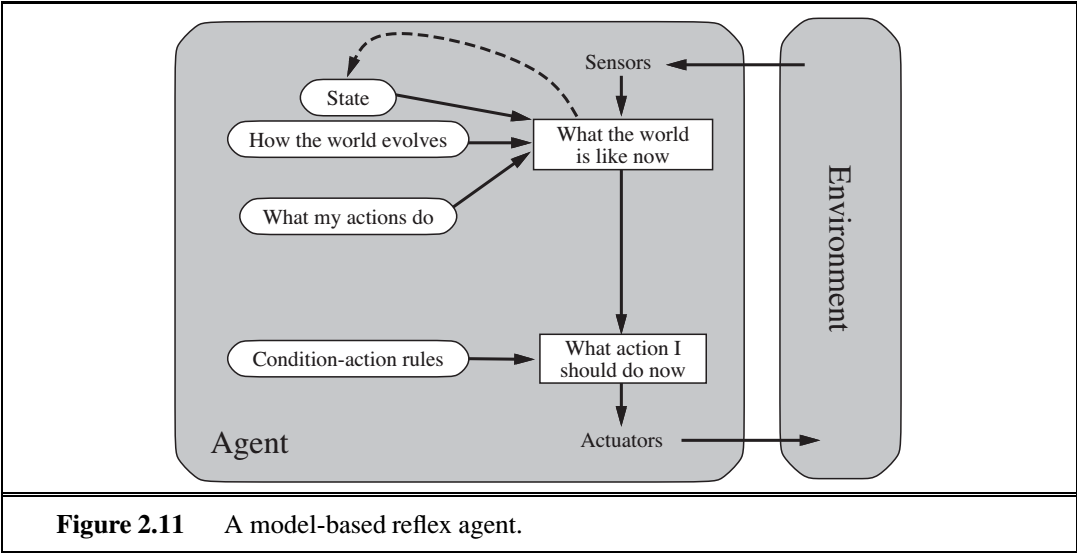
\includegraphics[scale=0.4]{img/refage.png}
\end{center}
The most effective way to handle partial observability is for the agent to keep track of the part of the world it can't see right now.

A stateful reflex agent has a world model consisting of:
\begin{itemize}
    \item
        a \textbf{belief state} that has information about the possible states the world may be in
    \item
        a \textbf{transition model} that updates the belief state based on sensor information and actions
\end{itemize}
The agent environment determines what the world model can be.

\bigbreak

In a fully observable, deterministic environment
\begin{itemize}
    \item
        we can observe the initial state and subsequent states are giben by the actions alone
    \item
        the belief state is a singleton set and the transition model is a function from states and actions to states: a \textbf{transition} function
\end{itemize}

In a fully observable, but stochastic environment
\begin{itemize}
    \item
        the belief state must deal with a set of possible states
    \item
        generalize the transition function to a \textbf{transition relation}
\end{itemize}

In a deterministic, but partially observable environment
\begin{itemize}
    \item
        the belief state must deal with a set of possible states
    \item
        we can use a transition function
    \item
        We need a \textbf{sensor model}, which predicts the influence of percepts on the belief state - during update
\end{itemize}

In a stochastic, partially observable environment
\begin{itemize}
    \item
        mix the ideas from the last two (sensor model + transition relation)
\end{itemize}
\end{comment}



\subsection{The Value of Information}
\textbf{Information value theory} enables an agent to choose what information to acquire.

\subsubsection{Example}
\begin{itemize}
    \item
        Oil company wants to buy one of \(n\) blocks of ocean-drill rights
    \item
        One of the blocks contains oil worth \(C\) dollar, while others are worthless
    \item
        Suppose seismologist offers the company results of a survey of block number 3, which indicates definitively wether the block contains oil
    \item
        How much should the company be willing to pay for the information?
\end{itemize}

With probability \(1/n\), the survey will indicate oil in block 3 and the company will buy block 3 for \(C/n\) dollars

 \(\Rightarrow Profit = C - C/n = (n-1)C/n\)

 With probability \(n-1)/n\), the survey will show that block contains no oil, in which case the company will buy a different block
 
 \(\Rightarrow Expected \ Profit = C/(n-1) - C/n = C/(n-1)n\) 

 Expected profit, given the survey information: \(\frac{1}{n} \times \frac{(n-1)C}{n} + \frac{n-1}{n} \times \frac{C}{n(n-1)} = C/n\)

 Therefore, the company should be willing to pay the seismologist up to \(C/n\) dollars for the information: the information is worth as much as the block itself.

 In general, the value of a given piece of information is defined to be the difference in expected value between best action before and after information is obtained.

\subsubsection{A general formula for perfect imformation}
We assume that exact evidence can be obtained about the value of some random variable \(E_j\) (that is, we learn \(E_j = e_j\), so the phrase \textbf{value of perfect information} (VPI) is used.

Let the agent's initial evidence be \(e\). Then the value of the current best action \(\alpha\) is defined by
\[EU(\alpha|e) = max_{a} \sum_{s'} P(Result(a) = s'|a, e) U(s')\]
and the value of the next best action (after the new evidence \(E_j = e_j\) is obtained) will be 
\[EU(\alpha_{e_j}|e, e_j) = max_a \sum_{s'} P(Result(a) = s' | a, e, e_j) U(s')\]
But \(E_j\) is a random variable whose value is currently unknown, so to determine the value of discovering \(E_j\), given current information \(e\) we must average over all possible values \(e_{jk}\) that we might discover, using our current beliefs about its value:
\[VPI_e(E_j) = (\sum_k P(E_j = ejk | e) EU(\alpha_{e_{jk}} | e, E_j = e_{jk})) - EU(\alpha|e)\]

\begin{center}
    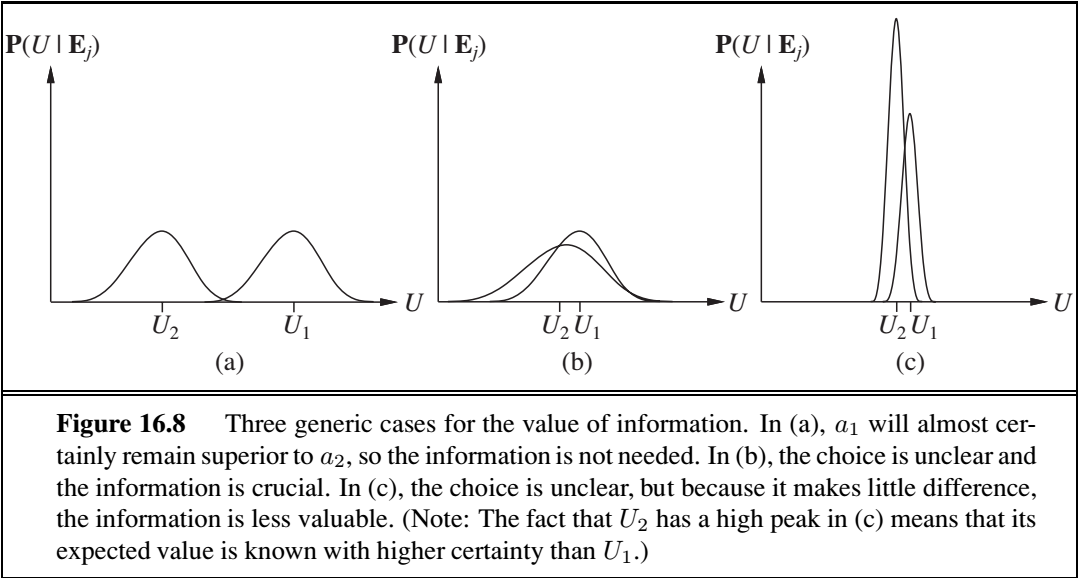
\includegraphics[scale=0.4]{img/vpi.png}
\end{center}

\begin{itemize}
    \item
        Suppose \(a_1\), \(a_2\) represent two different routes through mountain range
    \item
        (a)
        \begin{itemize}
            \item
                \(a_1\) nice and chill, \(a_2\) winding road, might snow as fuck and way might be blocked
            \item
                Clearly: \(U_1 > U_2\)
            \item
                Possibility to obtain satellite images
            \item
                Distribution of new expectations shows that, about 99.9\% of the time the plans won't change
        \end{itemize}
    \item
        (b)
        \begin{itemize}
            \item
                Choosing between two similar roads which could be blocked and we are carrying a seriously injured passenger 
            \item
                \(U_1\) and \(U_2\) are quite close
            \item
                Distributions show that sattelite information might change utilities drastically (because very broad)
        \end{itemize}
    \item
        (c)
        \begin{itemize}
            \item
                Choosing between two dirt roads in summertime, when blockage is unlikely (Utilities pretty close)
            \item
                Distributions show that additional information might quite likely change our plans
            \item
                But: The difference in utility is likely to be very small, so it isn't worth the effort
        \end{itemize}
\end{itemize}

\bigbreak

\textbf{In sum, information has value to the extent that it is likely to cause a change of plan and to the extent that the new plan will be significantly better than the old plan.}

\subsubsection{Implementation of an information-gathering agent}
A sensible agent should ask questions in a reasonable order, should avoid asking questions that are irrelevant, should take into account the importance of each piece of information in relation to its cost, and should stop asking questions when that is appropriate.

We assume that with each observable evidence variable \(E_j\), there is an associated cost, \(Cost(E_j)\). We assume that the result of the action \(Request(E_j)\) is that the next percept provides the value of \(E_j\).

\begin{center}
    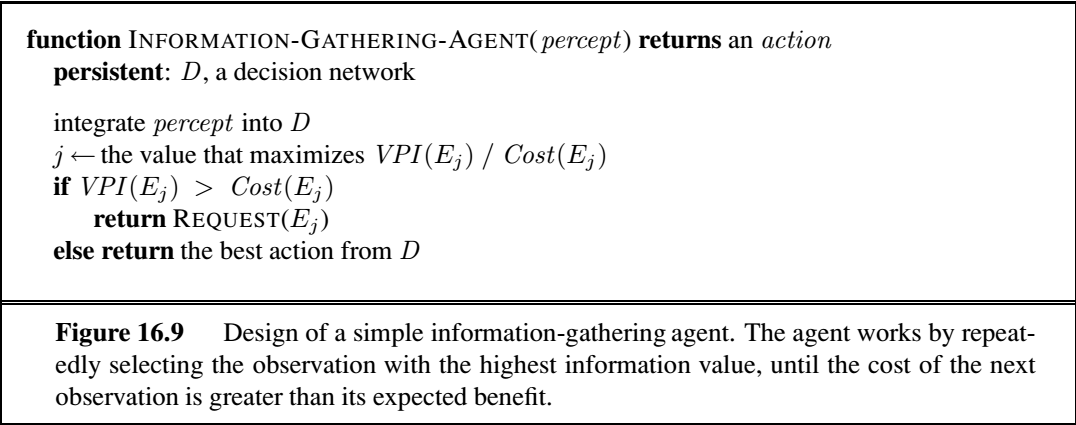
\includegraphics[scale=0.4]{img/vpiag.png}
\end{center}

Form of information gathering: \textbf{myopic}. The algorithm uses the VPI formula shortsightedly, calculating the value of information as if only a single evidence variable will be acquired. If there is no single evidence variable that will help a lot, a myopic agent might hastily take an action when it would have been better to request two or more variables first and then take actions.

\section{Temporal probability models (Probabilistic Reasoning Over Time)}
\subsection{States and observation}
We view the world as a series of snapshots, or \textbf{times slices}, each of which contains a set of random variables, some observable and some not. We will use \(X_t\) to denote the set of state variables at time \(t\), which are assumed to be unobservable, and \(E_t\) to denote the set of observable evidence variables. The observation time \(t\) is \(E_t = e_t\) for some set of values \(e_t\). The state sequence starts at \(t=0\).

\textit{Notation:} \(X_{a:b} = \) set of variables from \(X_a\) to \(X_b\).

\subsection{Transition and sensor models}
Two questions: 
\begin{itemize}
    \item
        How does the world evolve? (\(\rightarrow\) \textbf{transition model})
    \item
        How do evidence variables get their values (\(\rightarrow\) \textbf{sensor model})
\end{itemize}

\bigskip

The \textbf{transition model} specifies the probability distribution over the last state variables given the previous values, that is, \(P(X_t | X_{0:t-1})\).
\begin{itemize}
    \item
        Problem: the set \(X_{0:t-1}\) is unbound in the size as \(t\) increases
    \item
        Solution: \textbf{Markov assumption} - the current state depends only on a \textit{finite fixed number} of previous states  
    \item
        Processes satisfying this assumption are called \textbf{Markov processes} or \textbf{Markov chains} 
    \item
        Another problem: infinetly many possible values of \(t\). Do we need specify a different distribution for each time step?
    \item
        Another solution: We assume that changes in the world state are caused by a \textbf{stationary process}, which doesn't change over time (e.g. \(P(R_t | R_{t-1})\) is the same \(\forall t\))
\end{itemize}

\begin{center}
    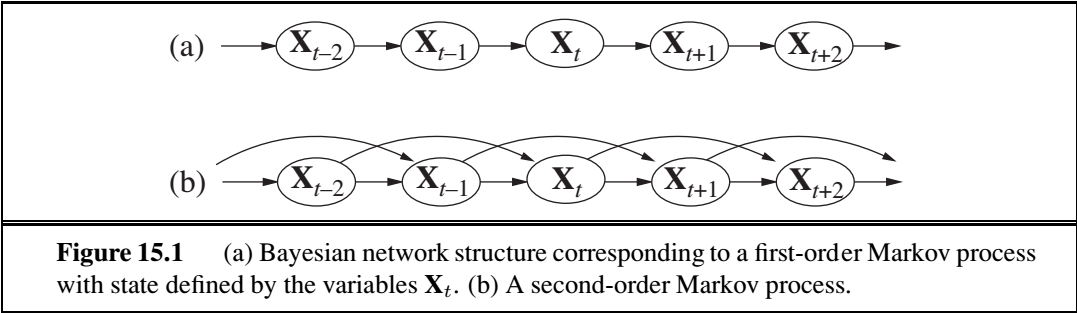
\includegraphics[scale=0.4]{img/markpro.png}
\end{center}

\bigbreak

The \textbf{sensor model} specifies, how evidences are generated (on which state variables they depend). We make the \textbf{sensor Markov assumption}:
\[P(E_t | X_{0:t}, E_{0:t-1}) = P(E_t | X_t)\]

\begin{center}
    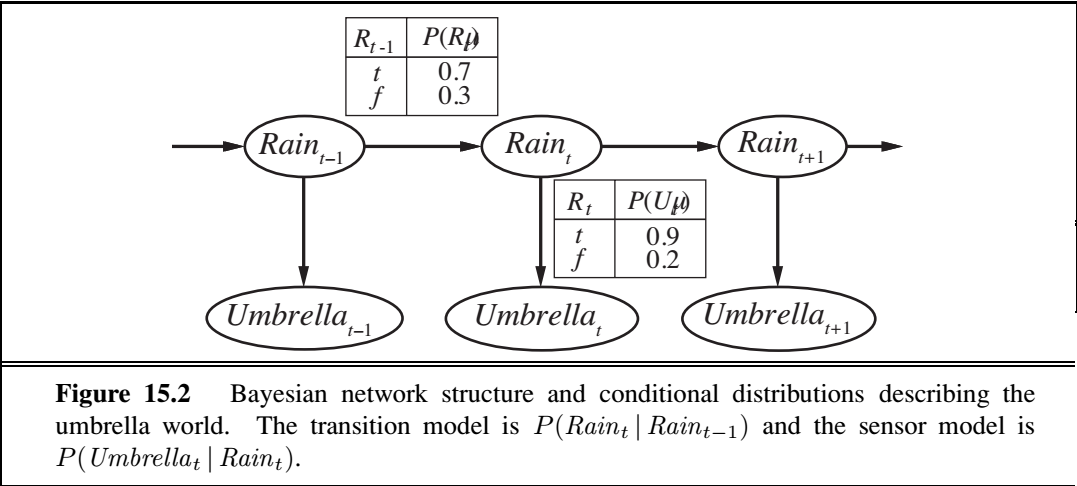
\includegraphics[scale=0.4]{img/transenmod.png}
\end{center}

Additionally, we need to specify an intial state probability \(P(X_0)\).

The complete joint probability distribution over all the variables is (for any \(t\), with first order Markov assumption) given by
\[P(X_{0:t}, E_{1:t}) = P(X_0) \prod_{i=1}^t P(X_i|X_{i-1}) P(E_i | X_i)\]
and consists of initial state probability, the transition model and the sensor model.

One problem with the first order Markov assumption is, that it might not model the real world apropriatly. Possible fixes:
\begin{itemize}
    \item
        Increase order of Markov process
    \item
        Augment state, e.g. \(Season_t\), \(Temp_t\), \(Pressure_t\) 
\end{itemize}

\subsection{Inference in Temporal Models}












\newpage
\section{Russel, Norvig: Artificial Neural Networks}
\subsection{Neural Network structures}
\begin{itemize}
    \item
        A link from unit \(i\) to \(j\) serves to propagate the activation \(a_i\) from \(i\) to \(j\)
    \item
        Each link has a numeric weight \(w_{i,j}\)
    \item
        Each unit has a dummy input \(a_0 = 1\) with an associated weight \(w_{0,j}\)
    \item
        Each unit \(j\) first computes a weighted sum of its inputs: \[in_j = \sum_{i=0}^n w_{i,j} a_i\]
    \item
        Then it applies an activation function \(g\) to this sum to derive the output:
        \[a_j = g(in_j) = g(\sum_{i=0}^n w_{i,j} a_i)\]
    \item
        Activation function: perceptron (hard) vs. sigmoid perceptron (soft) threshold
\end{itemize}
\subsection{Multilayer feed-forward neural networks}
\begin{itemize}
    \item
        Thinking of neural network as (vector) function \(h_w(x)\), which is fully parameterized by the weights \(w\) 
    \item
        As long as we can calculate the derivatives of such expressions with respect to the weights, we can use the gradient-descent loss-minimization method to train the network
\end{itemize}
\subsection{Learning in multilayer networks}
\begin{itemize}
    \item
        Loss function is additive across the components of the error vector.
        For the L2-Loss: \[\frac{\partial}{\partial w} Loss(w) = \frac{\partial}{\partial w} \abs{y-h_w(X)}^2 = \dots = \sum_k \frac\partial{\partial w} (y_k - a_k)^2\] 
    \item
        Each term in the final summation is the gradient of the loss for the \(k\)th output, computed as if the other outputs did not exist\\
        \(\Rightarrow\) we can decompose an \(m\)-output learning problem into \(m\) learning problems
    \item
        The error at the outer layer is clear, at hidden layers it is mysterious \(\Rightarrow\) backpropagate error 
    \item
        \dots
\end{itemize}
\subsubsection{Derivation}
\begin{itemize}
    \item
        We compute just the gradient for \(Loss_k = (y_k - a_k)^2\) at the \(k\)th output 
    \item
        The gradient w.r.t to weights connecting the hidden layer to the output layer will be zero exept for weights \(w_{j,k}\) that connect to the \(k\)th output unit
    \item
        \[\frac{\partial Loss_k}{\partial w_{j,k}} = -2(y_k -a_k) \frac{\partial a_k}{\partial w_{j,k}} = \dots = -a_j \Delta_k\]
        with \(\Delta_k = g'(in_k) \sum_j w_{k,j} \Delta_j\)
\end{itemize}
\end{document}

